\subsubsection{Répartition des éditions le long des séquences}
La distance totale laisse ouverte la question de la position des différences. Lorsque les extrémités des deux séquences coïncident, leur retrait réduit la longueur à traiter tout en conservant la distance. La figure~\ref{fig:methodes} compare cet effet sur un témoin humain et sur deux fenêtres homologues. Pour chaque méthode, huit processus mesurent chacun dix appels après échauffement. L’écart-type porte sur les huit moyennes de processus.
\chart{comparison/methodes_exactes.png}{Temps par appel sur un cœur EPYC, en millisecondes. Chaque case donne la moyenne de huit processus, puis l’écart-type et la demi-largeur de l’intervalle à 95\,\%. Le filet horizontal sépare le score seul du calcul du chemin. Pour chaque paire et chaque sortie, le minimum apparaît en gras. La teinte suit le logarithme du rapport à ce minimum.}{fig:methodes}{bench/repeated/bands.py}

Sur le témoin de 100\,000 bases, les substitutions touchent un seul bloc central de 128 bases. Après retrait des extrémités, ce bloc suffit pour retrouver les 72 éditions de l’alignement optimal. Le retrait des extrémités fait passer le temps du calcul en bande de \(54{,}661\pm0{,}055\) à \(0{,}1038\pm0{,}0010\)\,ms sur un cœur EPYC. Les deux fenêtres homologues de 50\,000 bases commencent par 207 bases identiques et se terminent par deux bases différentes. Il reste donc 49\,793 bases de chaque côté après retrait du préfixe. Le même traitement fait passer le temps de \(230{,}599\pm0{,}046\) à \(229{,}420\pm0{,}067\)\,ms.

Dans A*PA2, la version simple exploite l’écart de longueur pour minorer le coût restant. La version complète ajoute une heuristique fondée sur des correspondances entre fragments. Les deux versions rendent le chemin. Sur la paire synthétique de 20\,000 bases à 10\,\% d'éditions injectées, les temps moyens valent \(0{,}875\pm0{,}008\)\,ms pour le mode simple, \(1{,}534\pm0{,}007\)\,ms pour le mode complet et \(3{,}736\pm0{,}022\)\,ms pour WFA2 en coût seul. Ces trois temps portent sur la même paire, avec des sorties différentes selon la bibliothèque.

\synthese{Sur huit blocs appariés, le retrait des extrémités accélère le calcul en bande d’un facteur 526,6 sur le témoin (IC à 95\,\% de 522,2 à 530,9). Sur les fenêtres homologues, ce facteur atteint seulement 1,0051 (de 1,0048 à 1,0055).}

\subsection{Validation et coût de la reconstruction}\label{sec:reconstruction}
Un score indique combien d’éditions sont nécessaires. Pour restituer un alignement, il faut aussi trouver une suite d’opérations de ce coût qui transforme toute la première séquence en la seconde. Les témoins de WFA2 et de QuickEd permettent de contrôler ces deux propriétés. Les mesures de Hirschberg et de BiWFA montrent ensuite ce que la reconstruction ajoute en temps et en mémoire, jusqu’aux fenêtres du chromosome~21.

\subsubsection{Contrôle des scores et des chemins}\label{sec:quicked}
Les essais de portabilité comparent la version publiée de WFA2-lib à une variante qui accepte les lectures de huit octets à toute adresse et ajuste le curseur de l’allocateur. Sur EPYC, GCC~11.5 produit le même code machine pour l’extension du front, mais les fichiers objets de l’allocateur diffèrent. Les 800 appels restituent les scores attendus. Sur la paire de 20\,000 bases à 10\,\% d’éditions injectées, le rapport des temps de la variante portable et de la version publiée vaut 0,997 (IC à 95\,\% de 0,992 à 1,002). Pour chacune des cinq paires, l’intervalle contient 1.

Lors de la reconstruction, le programme copie le CIGAR par blocs d’octets et borne la dernière écriture au nombre d’octets restants. Des tests instrumentés par ASan et UBSan couvrent 33 longueurs pour chacun des huit décalages de l’adresse de sortie. Sur EPYC, le rejeu a validé 48\,384 chemins de la cohorte virale. Sur le même nœud, le rapport apparié des temps de reconstruction de BiWFA avec et sans cette écriture bornée vaut 1,0002 sur huit blocs (IC à 95\,\% de 0,9908 à 1,0097).

Le contrôle de QuickEd porte d’abord sur la largeur de la bande. QuickEd estime une borne de coût par fenêtres et la transmet à la reconstruction de Hirschberg. Si tous les chemins optimaux sortent de la bande, le meilleur chemin qu’elle contient coûte davantage. Deux témoins périodiques de 512 bases ont une distance globale de 128. En imposant \(\lvert i-j\rvert\le63\) à une DP scalaire indépendante, les deux scores deviennent 133 et 129. Une demi-largeur de 64 suffit pour retrouver 128 dans chaque cas.

Le second contrôle porte sur la lecture des prédécesseurs pendant la reconstruction. Sur le M1 Pro, la version amont de QuickEd~1.2 renvoie 954 et 450 pour ces mêmes témoins. La borne transmise à Hirschberg vaut déjà 128 dans les deux cas. Le défaut observé vient de la remontée du chemin au bord d'un bloc, où un prédécesseur se trouve hors des bits stockés. Sur EPYC avec GCC~11 en compilation native, la première estimation vaut 130. Les deux scores amont valent alors 128. Lors de la remontée, le contrôle d'indice vérifie que chaque prédécesseur appartient au bloc avant de lire son bit.

Dans QuickEd avec contrôle du chemin, l'adaptateur rejoue le CIGAR et compare son coût au score global d'Edlib. En cas d'écart, il relance Hirschberg avec une bande plus large. Si la dernière tentative échoue, il renvoie le score d'Edlib en indiquant son origine.

Sur deux autres témoins EPYC, QuickEd amont renvoie 506 au lieu de 128 et 760 au lieu de 256, dans chacun des 80 appels par témoin. Pour les dix entrées chronométrées, le contrôle du chemin réussit dès la première tentative. Un test qui impose artificiellement une première bande de 1\,\% déclenche un nouveau calcul et ramène le candidat de 896 à la distance vérifiée 384.

\chart{comparison/quicked.png}{Scores et durées sur témoins contrôlés et entrées génomiques. Les 80 appels par méthode et par entrée sont répartis entre huit processus.}{fig:quicked}{bench/quicked/measure.py}
\FloatBarrier
La figure~\ref{fig:quicked} donne le coût des chemins témoins et le temps de vérification sur les entrées génomiques. Sur les paires de 20\,000 bases à 2, 5 et 10\,\%, les temps moyens avec contrôle du chemin sont respectivement \(2{,}375\pm0{,}008\), \(2{,}996\pm0{,}010\) et \(4{,}521\pm0{,}011\)\,ms. Les vérifications du coût et du chemin font partie du chronométrage.

\synthese{Sur EPYC, les 800 CIGAR vérifiés consomment les deux chaînes et retrouvent le coût de référence. L’adaptateur élargit la bande lorsque le coût du chemin rejoué diffère du score d’Edlib.}

\subsection{Reconstruction en mémoire linéaire}
Une trace optimale passe par une colonne de la ligne médiane \(h=\lfloor m/2\rfloor\). Le principe de coupe de Hirschberg~\cite{hirschberg}, initialement formulé pour une plus longue sous-séquence commune, s'applique aux coûts unitaires d'édition. Une passe avant calcule \(F_j=d(A_{1:h},B_{1:j})\). Une passe en sens inverse calcule \(G_{n-j}=d(A_{h+1:m},B_{j+1:n})\). En coupant un chemin optimal à la ligne \(h\), puis en concaténant deux solutions optimales pour cette coupe, on obtient
\[
 d(A,B)=\min_{0\le j\le n}(F_j+G_{n-j}).
\]
Le noyau retient une colonne minimisante et résout récursivement les deux rectangles. Il place la plus courte chaîne en colonnes et réutilise les deux mêmes tableaux dans les appels enfants. Les scores occupent \(8(\min(m,n)+1)\) octets, auxquels s'ajoutent la pile de profondeur logarithmique et le CIGAR de sortie. À chaque niveau, la somme des aires décroît avec les hauteurs des rectangles. Le travail reste en \(O(mn)\).
\chart{cpu/trace_lineaire.png}{Chaque segment relie les deux reconstructions sur le même préfixe. Les barres horizontales et verticales donnent la dispersion et l'IC à 95\,\% sur 31 processus pour la durée et le pic RSS respectivement.}{fig:trace}{bench/repeated/measure.py}
La figure~\ref{fig:trace} utilise des préfixes d'une même paire. À 2\,000 bases, la matrice complète prend \(5{,}778\pm0{,}281\)\,ms et Hirschberg \(8{,}907\pm0{,}039\)\,ms. À 8\,000 bases, les deux chemins coûtent 203 éditions. Les temps passent à \(99{,}406\pm0{,}571\) et \(141{,}898\pm0{,}510\)\,ms. Les maxima du RSS sur les 31 processus sont respectivement 253\,424 et 6\,940\,Kio.

À la limite dense de 20\,000 bases par chaîne, les six reconstructions sur Grace et GH200 réalisent 454 éditions. Sur le GPU, les lignes de score et l'index occupent 480\,024 octets en coût seul. La matrice de trace et l'index occupent \(4(20\,001)^2+16(20\,001)=1\,600\,480\,020\) octets. En allongeant d'une base la première ou la seconde chaîne, Hirschberg retrouve respectivement 453 et 455 éditions.

\synthese{À 25\,000 bases, Hirschberg reconstruit un chemin de 531 éditions en \(1{,}38331\pm0{,}00107\)\,s. Les coupes évitent de conserver toute la matrice au prix de passes supplémentaires sur les préfixes.}

\subsubsection{Fronts bidirectionnels et reconstruction du chemin}\label{sec:biwfa}
Hirschberg choisit la coupe sur une ligne fixée à l’avance. Dans BiWFA, de Marco-Sola et ses coauteurs, la rencontre de deux fronts détermine la coupe~\cite{biwfa}. Pour les coûts unitaires de l’expérience, les fronts partent des extrémités opposées de l’alignement et cherchent un chevauchement sur une même diagonale. Une jonction optimale \((i,j)\) scinde les chaînes \(A,B\) en deux sous-problèmes dont les coûts se composent,
\[
 d(A,B)=d\bigl(A[0:i],B[0:j]\bigr)+d\bigl(A[i:m],B[j:n]\bigr).
\]
Le mode score s'arrête lorsque la jonction ou l'extrémité est atteinte. Pour restituer le chemin, BiWFA résout les sous-problèmes et assemble leurs opérations. Avec \(s=d(A,B)\ge1\) et \(L=\max(m,n)\), la borne de temps est \(O(Ls)\) et celle de mémoire de travail des fronts \(O(s)\). Le RSS comprend aussi les entrées, les copies et le chemin rendu. La version mesurée utilise un front unidirectionnel auxiliaire sur les petits sous-problèmes.

L'algorithme~\ref{alg:biwfa} décrit cette décomposition pour le coût unitaire. La figure~\ref{fig:jonction} donne un chemin de coût deux. La substitution précède la jonction et l'insertion la suit.
\begin{algorithm}[htbp]
\caption{Reconstruction d'un chemin par fronts bidirectionnels}\label{alg:biwfa}
\begin{algorithmic}[1]
\Require Strings \(A,B\), unit edit costs
\Ensure Optimal operation sequence \(P\)
\If{\Call{BaseCase}{$A,B$}}
  \State \Return \Call{UnidirectionalTrace}{$A,B$}
\EndIf
\State \((i,j)\gets\Call{OptimalOverlap}{A,B}\) \Comment{forward and reverse wavefronts}
\State \(P_L\gets\Call{BiWFA}{A[0:i],B[0:j]}\)
\State \(P_R\gets\Call{BiWFA}{A[i:m],B[j:n]}\)
\State \Return \(P_L\mathbin{\Vert}P_R\)
\end{algorithmic}
\end{algorithm}
\schema{jonction}{Une jonction optimale sépare la substitution du préfixe et l'insertion du suffixe sur deux chaînes courtes.}{fig:jonction}{src/libraries/wfa2/wfa_adapter.c}

\begin{figure}[htbp]\centering
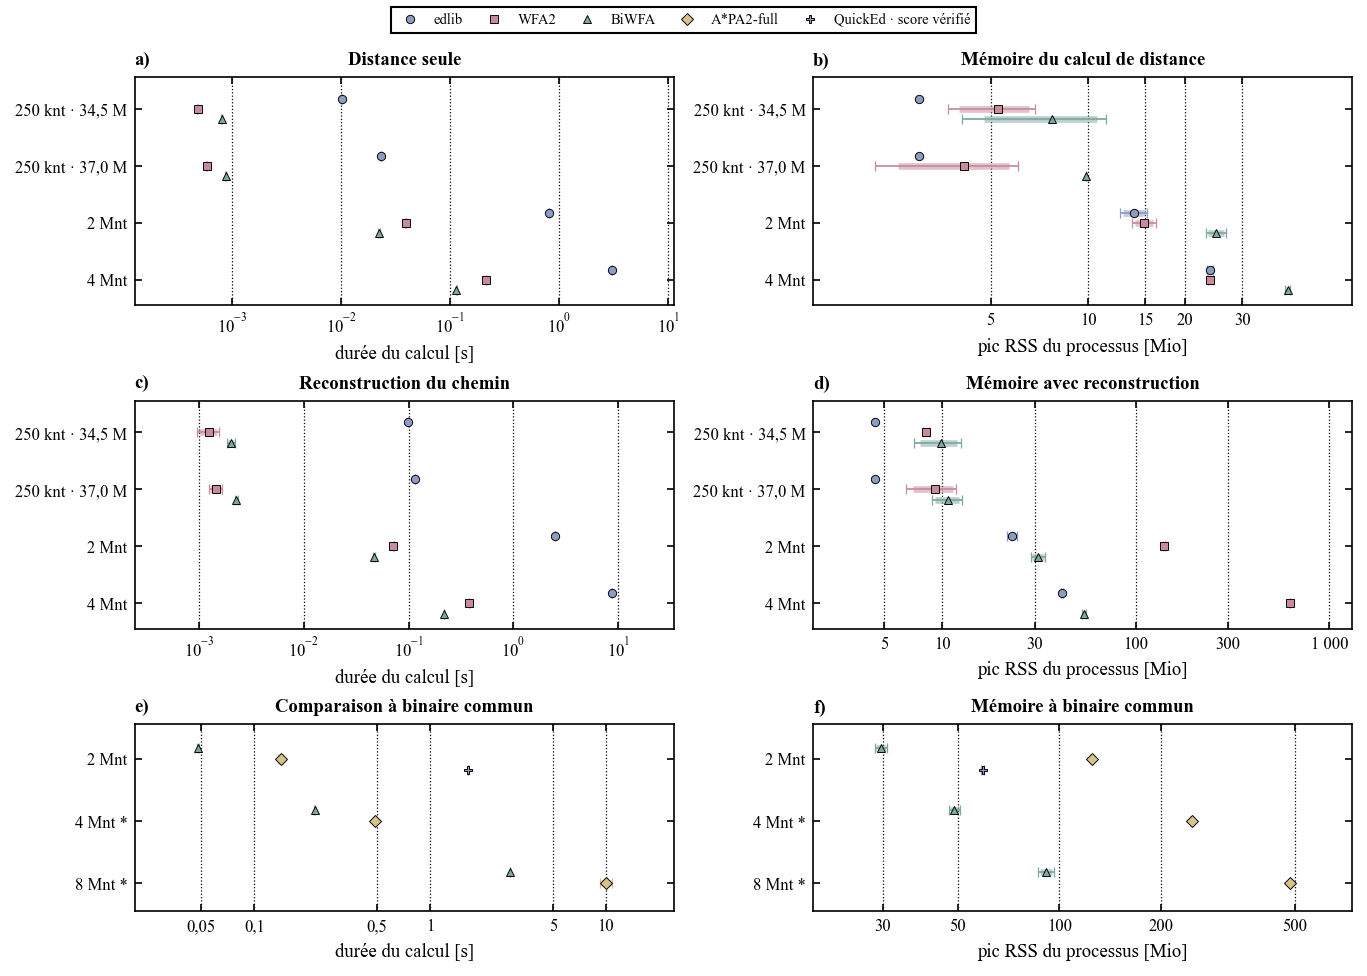
\includegraphics[width=.97\linewidth,height=.44\textheight,keepaspectratio]{../figures/comparison/biwfa_humain.png}
\sourcefig{bench/human/algorithms/study.py}
\caption{Les rapports de temps et de mémoire entre WFA2 et BiWFA distinguent le score et la reconstruction sur un cœur EPYC. Un rapport supérieur à un favorise BiWFA. Le tableau donne les temps d’une seconde allocation. Le terme « échéance » indique un arrêt du processus à 120\,s, chauffe comprise.}\label{fig:biwfa}
\end{figure}
La figure~\ref{fig:biwfa} compare des appels complets après échauffement, sur cinq processus indépendants par cas. Les fenêtres se recouvrent en partie. À quatre millions de bases et \(s=12\,482\), BiWFA rend le chemin en \(218{,}72\pm1{,}00\)\,ms avec un pic RSS moyen de 54,02\,Mio. WFA2 unidirectionnel prend \(375{,}90\pm2{,}35\)\,ms et 627,02\,Mio pour le même résultat. La moyenne des rapports appariés de temps vaut 1,719 (IC à 95\,\% de 1,707 à 1,730). Sur les deux loci de 250\,000 bases, WFA2 unidirectionnel termine en \(1{,}25\pm0{,}24\) et \(1{,}45\pm0{,}16\)\,ms. BiWFA prend \(2{,}03\pm0{,}13\) et \(2{,}28\pm0{,}06\)\,ms.

\begin{samepage}
Pour le score seul, le classement en mémoire s’inverse (panneaux a et b). À quatre millions de bases, le score seul occupe 23,87\,Mio avec WFA2, qui réutilise ses fronts en mémoire circulaire, et 41,46\,Mio avec BiWFA. Un relevé séparé sur la fenêtre de deux millions de bases compte 62 choix de sous-intervalle pendant la reconstruction BiWFA et aucun en mode score seul.\par
\end{samepage}

Un second banc utilise le même cœur pour les méthodes comparées à taille fixée. A*PA2 et BiWFA rendent le chemin. L'adaptateur QuickEd vérifie son chemin en interne et rend le score. À huit millions de bases, A*PA2 de Groot Koerkamp~\cite{astar} prend \(10{,}040\pm0{,}628\)\,s et BiWFA \(2{,}845\pm0{,}008\)\,s. À deux millions, QuickEd de Doblas et ses coauteurs~\cite{quicked}, avec contrôle du chemin, prend \(1{,}6391\pm0{,}0002\)\,s. Les processus QuickEd sur quatre et huit millions de bases atteignent la limite de 120\,s, lecture et échauffement compris.

\synthese{Sur la fenêtre de quatre millions de bases, le pic RSS de WFA2 pour restituer le chemin vaut 11,61 fois celui de BiWFA en moyenne sur les cinq rapports appariés. Les deux méthodes donnent le même coût.}

\subsubsection{Alignement du bras long du chromosome humain}\label{sec:bras}
Quatre fenêtres emboîtées du bras long du chromosome 21 partagent la même borne gauche, la base 14\,000\,100 de GRCh38 en coordonnées commençant à zéro. Leurs longueurs de référence valent 8, 16, 24 et 32 millions de bases. Leurs distances globales valent respectivement 47\,493, 89\,448, 133\,991 et 266\,220 éditions. Les chemins optimaux peuvent changer quand la borne droite se déplace. La soustraction de deux scores emboîtés ne suffit donc pas à localiser les éditions.

La fenêtre de 32 millions de bases contient 50\,160 caractères \texttt{N} dans GRCh38. CHM13 contient 31\,347 bases de plus et aucun \texttt{N}. Transformer la première chaîne en la seconde impose au moins une substitution ou une délétion pour chacun des \texttt{N}, ainsi qu'au moins 31\,347 insertions. Ces opérations distinctes donnent la borne \(d\ge50\,160+31\,347=81\,507\) pour les chaînes déposées.

\chart{comparison/bras_chromosome_biwfa.png}{BiWFA et WFA2 calculent le score sur quatre fenêtres emboîtées du bras long du chromosome 21. BiWFA restitue aussi un chemin sur chaque fenêtre. Les deux mesures d'Edlib (score seul et chemin) portent sur la fenêtre de 8~Mnt.}{fig:bras}{bench/human/algorithms/arm.py}
Les quatre tailles de la figure~\ref{fig:bras} occupent chacune un cœur distinct de l’EPYC. Les méthodes se succèdent sur ce cœur dans un ordre tiré par bloc. Chaque cas comporte cinq processus après échauffement. À 32 millions de bases, BiWFA calcule le score en \(45{,}62\pm0{,}22\)\,s et restitue le chemin en \(89{,}77\pm0{,}11\)\,s. Le pic RSS moyen atteint respectivement 272,83 et 311,17\,Mio. WFA2 unidirectionnel donne le score en \(102{,}04\pm0{,}91\)\,s avec 143,81\,Mio. Les fronts bidirectionnels se rejoignent avant que l'un d'eux atteigne le score total. Le gain en temps coïncide ici avec une hausse du pic résident.

\synthese{La restitution du chemin par BiWFA prend \(2{,}876\pm0{,}023\)\,s sur 8 millions de bases. Entre 8 et 32 millions de bases, la distance augmente d’un facteur 5,61 et le temps moyen d’un facteur 31,2. Ces fenêtres emboîtées font varier à la fois la longueur et la distance.}

